\documentclass[two column, twoside, a4paper]{article}

\usepackage[utf8]{inputenc}
\usepackage{dblfloatfix}
\usepackage{subcaption}
\usepackage{float}
\usepackage[backend=biber, maxbibnames=3, style=nature, autocite=inline]{biblatex}
\usepackage[polish]{babel}
\usepackage[T1]{fontenc}
\usepackage{fancyhdr}
\usepackage{titlesec}
\usepackage{blindtext}
\usepackage{gensymb}
\usepackage{cuted}
\usepackage{tikz}
\usepackage[most]{tcolorbox}
\usepackage[columnsep = 0.7cm,
	        lmargin = 0.6in,
	        rmargin = 0.6in,
	        tmargin = 0.5in,
	        bmargin = 0.65in,
	        headsep = \baselineskip]{geometry}

\addbibresource{$BIB}

% Custom commands
\newcommand*\circled[1]{\tikz[baseline=(char.base)]{
            \node[shape=circle,draw,inner sep=2pt, color = orange!90!white] (char) {#1};}}

% Section Formatting
\titleformat{\section}
{\sc \bfseries \Large}
{}
{0em}
{}[\titlerule]

\titleformat{\subsection}
{\bfseries \large}
{}
{0em}
{}

\titleformat{\subsubsection}
{\bfseries}
{}
{0em}
{}

% Box formatting
\tcbset{sharp corners, colback=white, enhanced, boxrule = 1pt, coltitle = orange!90!white, colbacktitle = orange!15!white, colframe= black!50!white}

\pagestyle{fancy}
\fancyhf{}
\fancyhead[RE, LO]{Szkoła Główna Gospodarstwa Wiejskiego}
\fancyhead[LE, RO]{Biotechnologia, semerstr V}
\fancyfoot[RE, LO]{Jakub J. Guzek}
\fancyfoot[LE, RO]{\thepage}
\fancyfoot[CE,CO]{Inżynieria Genetyczna}
\renewcommand{\footrulewidth}{0.05pt}

\begin{document}

\begin{strip}
	{\sc \bfseries \LARGE \fontfamily{phv}\selectfont Otrzymanie pomidora odpornego na infekcję \textit{Phytophthora capsici} metodą CRISPR/Cas9.} \vspace{\baselineskip}

{\bfseries \large Jakub J. Guzek}

{Szkoła Główna Gospodarstwa Wiejskiego. Biotechnologia, Semestr V, nr. albumu: 195528}\vspace{\baselineskip}

\hrule\vspace{\baselineskip}

	\textbf{\textsf{Choroby roślin powodują co roku ogromne straty gospodarcze. Nierzadko cała uprawa zostaje zmarnowana na skutek zakażenia patogenem. Rozwiązaniem tego problemu jest otrzymywanie odmian roślin odpornych na działanie tych patogenów. Jednak tradycyjne metody selekcjonowania nowych odmian zawodzą i nie dają długotrwałych rezultatów w wypadku niektórych chorób. Współcześnie dzięki metodom transformacji roślin i ukierunkowanej mutagenezy (genome-editing) możliwe jest otrzymanie odpornych odmian łatwiej i skuteczniej niż wcześniej. W tym projekcie opisuję proces otrzymywania odmiany pomidora odpornej na infekcję \textit{Phytophthora capsici}, przy użyciu transformacji roślin za pomocą \textit{A. tumefaciens} i metody edycji genomu CRISPR-Cas9}}\vspace{\baselineskip}

\hrule

\end{strip}

\textit{Phytophthora capsici} jest patogennym grzybem należącym do Lęgniowców (ang. \textit{oomycetes}) atakującym wiele rodzajów roślin. Najważniejszymi gospodarczo roślinami, na których grzyb ten pasożytuje są: ziemniak (\textit{Solanum tuberosum}), papryka (\textit{Capsicum annuum}) i pomidor (\textit{Solanum lycopersicum})\autocite{Lamour2012}. Jest to najbardziej destrukcyjny patogen \textit{C. annuum}, powodujący stratę ponad stu milionów dolarów rocznie w skali świata\autocite{Barchenger2018}. \textit{P. capsici} powoduje także wielomilionowe straty w uprawach pomidora, będącego drugim najbardziej konsumowanym warzywem na świecie.

Szeroki zakres żywicieli, duża różnorodność genetyczna, długowieczne zarodniki i odporność niektórych odmian na fungicydy czynią z \textit{P. capsici} groźny i trudny w opanowaniu problem w uprawach roślin. Nierzadko pole zakażone tym patogenem wymaga osuszenia na cały sezon aby w pełni pozbyć się z niego zarodników, które podatne są tylko na brak wody\autocite{Lamour2012}. Co więcej konwencjonalne metody otrzymywania odpornych na chorobę odmian roślin, oparte na selekcji hodowlanej nie sprawdzają się w tym wypadku ponieważ trudno jest otrzymać rośliny odporne na wszystkie szczepy patogenu. Udaje się jednak w ten sposób otrzymać linie odporne na poszczególne szczepy\autocite{Sy2005}. Wynika to z wysokiego polimorfizmu sekwencji jednego z efektorów wirulencji u rodzaju \textit{Phytophthora}\autocite{Chen2019}. Z tego powodu, atrakcyjne wydają się oparte na inżynierii genetycznej metody otrzymania odpornych odmian.

Zidentyfikowane zostały geny i białka związane z odpornością lub podatnością na \textit{P. capsici}, takie jak np. pochodzący z dzikiego ziemniaka (\textit{Solanum bulbocastanum}) gen RB (Fig. \ref{fig::c_annuum})\autocite{Song2003, Bagga2019}, białka ROP (\textit{Rho-related GTPases of Plants})\autocite{Yang2020}, czy też gen SlDMR6, którego wyciszenie powoduje powstanie roślin odpornych na szeroki zakres patogenów, w tym na \textit{P. capsici}\autocite{deToledoThomazella2016}.

W niniejszej pracy opisane jest otrzymanie linii pomidora, odpornego na infekcję \textit{P. capsici}. W pierwszej kolejności zaprezentowane jest otrzymanie konstruktów zawierających: (1) sekwencję kodującą białko Cas9 i gRNA, mające wprowadzić mutacje w rejonie kodującym genu SlDMR6. (2) sekwencję genu RB (haplotyp RB). Następnie transformacja roślin poszczególnymi konstruktami i otrzymanie stabilnych linii zawierających pożądane czynniki odporności, a na koniec ocena stopnia odporności poszczególnych linii na infekcje.

\begin{figure}[tp]
\begin{tcolorbox}
	\centering
	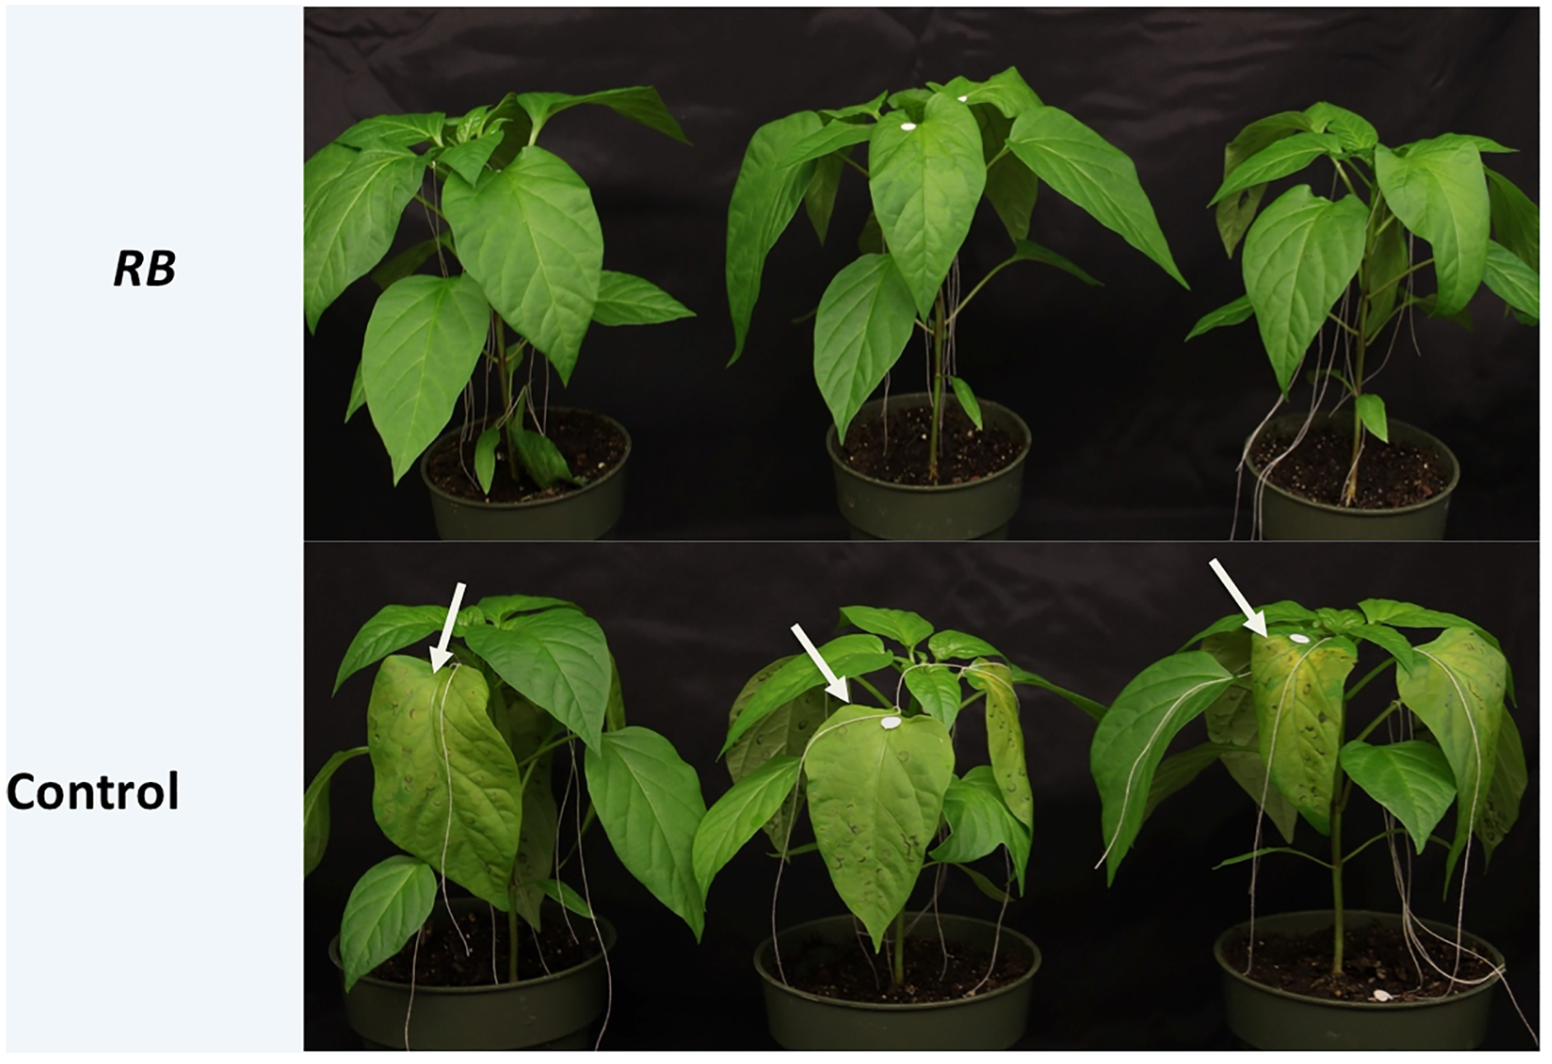
\includegraphics[width=\textwidth]{./figures/c_annuum.png}
	\caption{Fenotyp liści \textit{C. annuum} 48h po infekcji \textit{P. capsici}. Rośliny oznaczone RB posiadają wbudowane T-DNA z genem RB (haplotyp RB). Rośliny oznaczone Control posiadają wbudowany pusty wektor. Widać, że posiadające transgen roślinny są do pewnego stopnia odporne na infekcję. (Na podstawie: Bagga 2019)}\label{fig::c_annuum}
\end{tcolorbox}
\end{figure}

\section{Materiały i metody}

\subsection{Otrzymanie konstruktu CRISPR/Cas9}

Sekwencja gRNA została zaprojektowana aby wprowadzać mutacje w eksonie 2 i 3 genu SlDMR6 przy użyciu internetowego narzędzia CRISPR-P v2.0\autocite{Lei2014}. Oligonukleotydy z pożądanymi sekwencjami gRNA zostały zamówione od \textsf{Thermo Fisher Scientific}. Sekwencje gRNA i gen kodujący Cas9 zostały zinsertowane do wektorów pENTR\texttrademark/D-TOPO (Fig. \ref{fig::pENTR_D-TOPO}) przy użyciu kitu (pENTR™/D-TOPO™ Cloning Kit, with One Shot™ TOP10 Chemically Competent E. coli, \textsf{Invitrogen\texttrademark}).

Dla sekwencji kodującej gRNA został użyty promotor U6-26 z \textit{A. thaliana}, a dla genu Cas9, promotor 2 x 35S. gRNA, endonukleaza Cas9 oraz sekwencje promotorów zostały wklonowane do wektora pPZP200 (Fig. \ref{fig::pPZP200}) przy użyciu klonowania Gateway (MultiSite Gateway™ Pro Plus, for flexible cloning of up to four DNA fragments into a Gateway™ destination vector, \textsf{Thermo Fisher Scientific}). Metoda analogiczna do tej zastosowanej przed \textit{de Toledo Thomazella i wspł.}\autocite{deToledoThomazella2016}.

 \begin{figure*}[bp]
	 \begin{tcolorbox}
		 \centering
		 \begin{subfigure}[b]{0.52\textwidth}
			 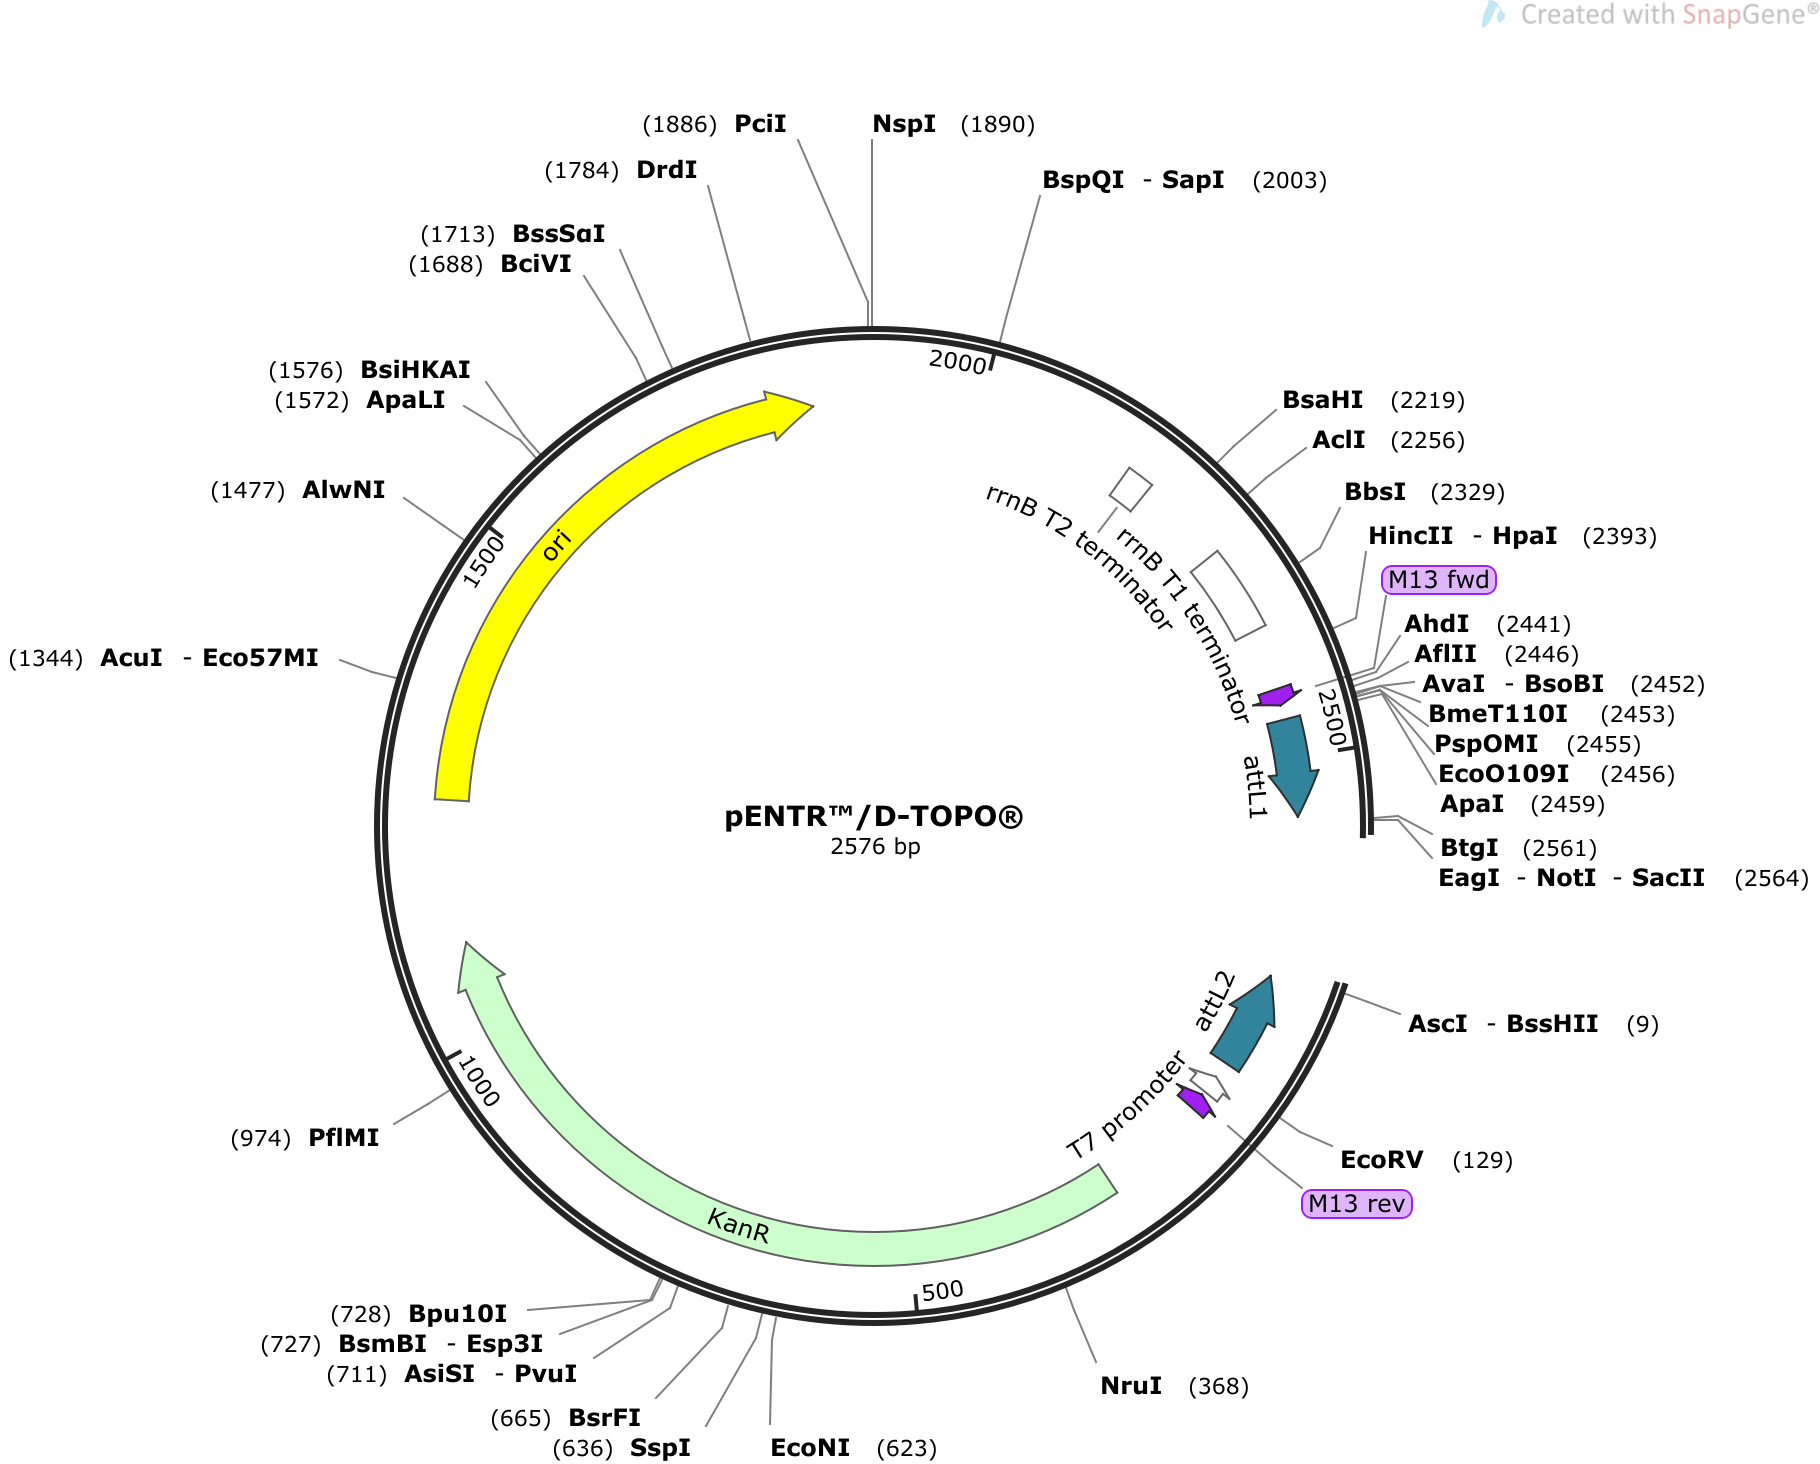
\includegraphics[width=\textwidth]{./figures/pENTR_D-TOPO.png}
		\caption{Wektor pENTR\texttrademark/D-TOPO}\label{fig::pENTR_D-TOPO}
		\end{subfigure}
		\hfill
		 \begin{subfigure}[b]{0.4375\textwidth}
			 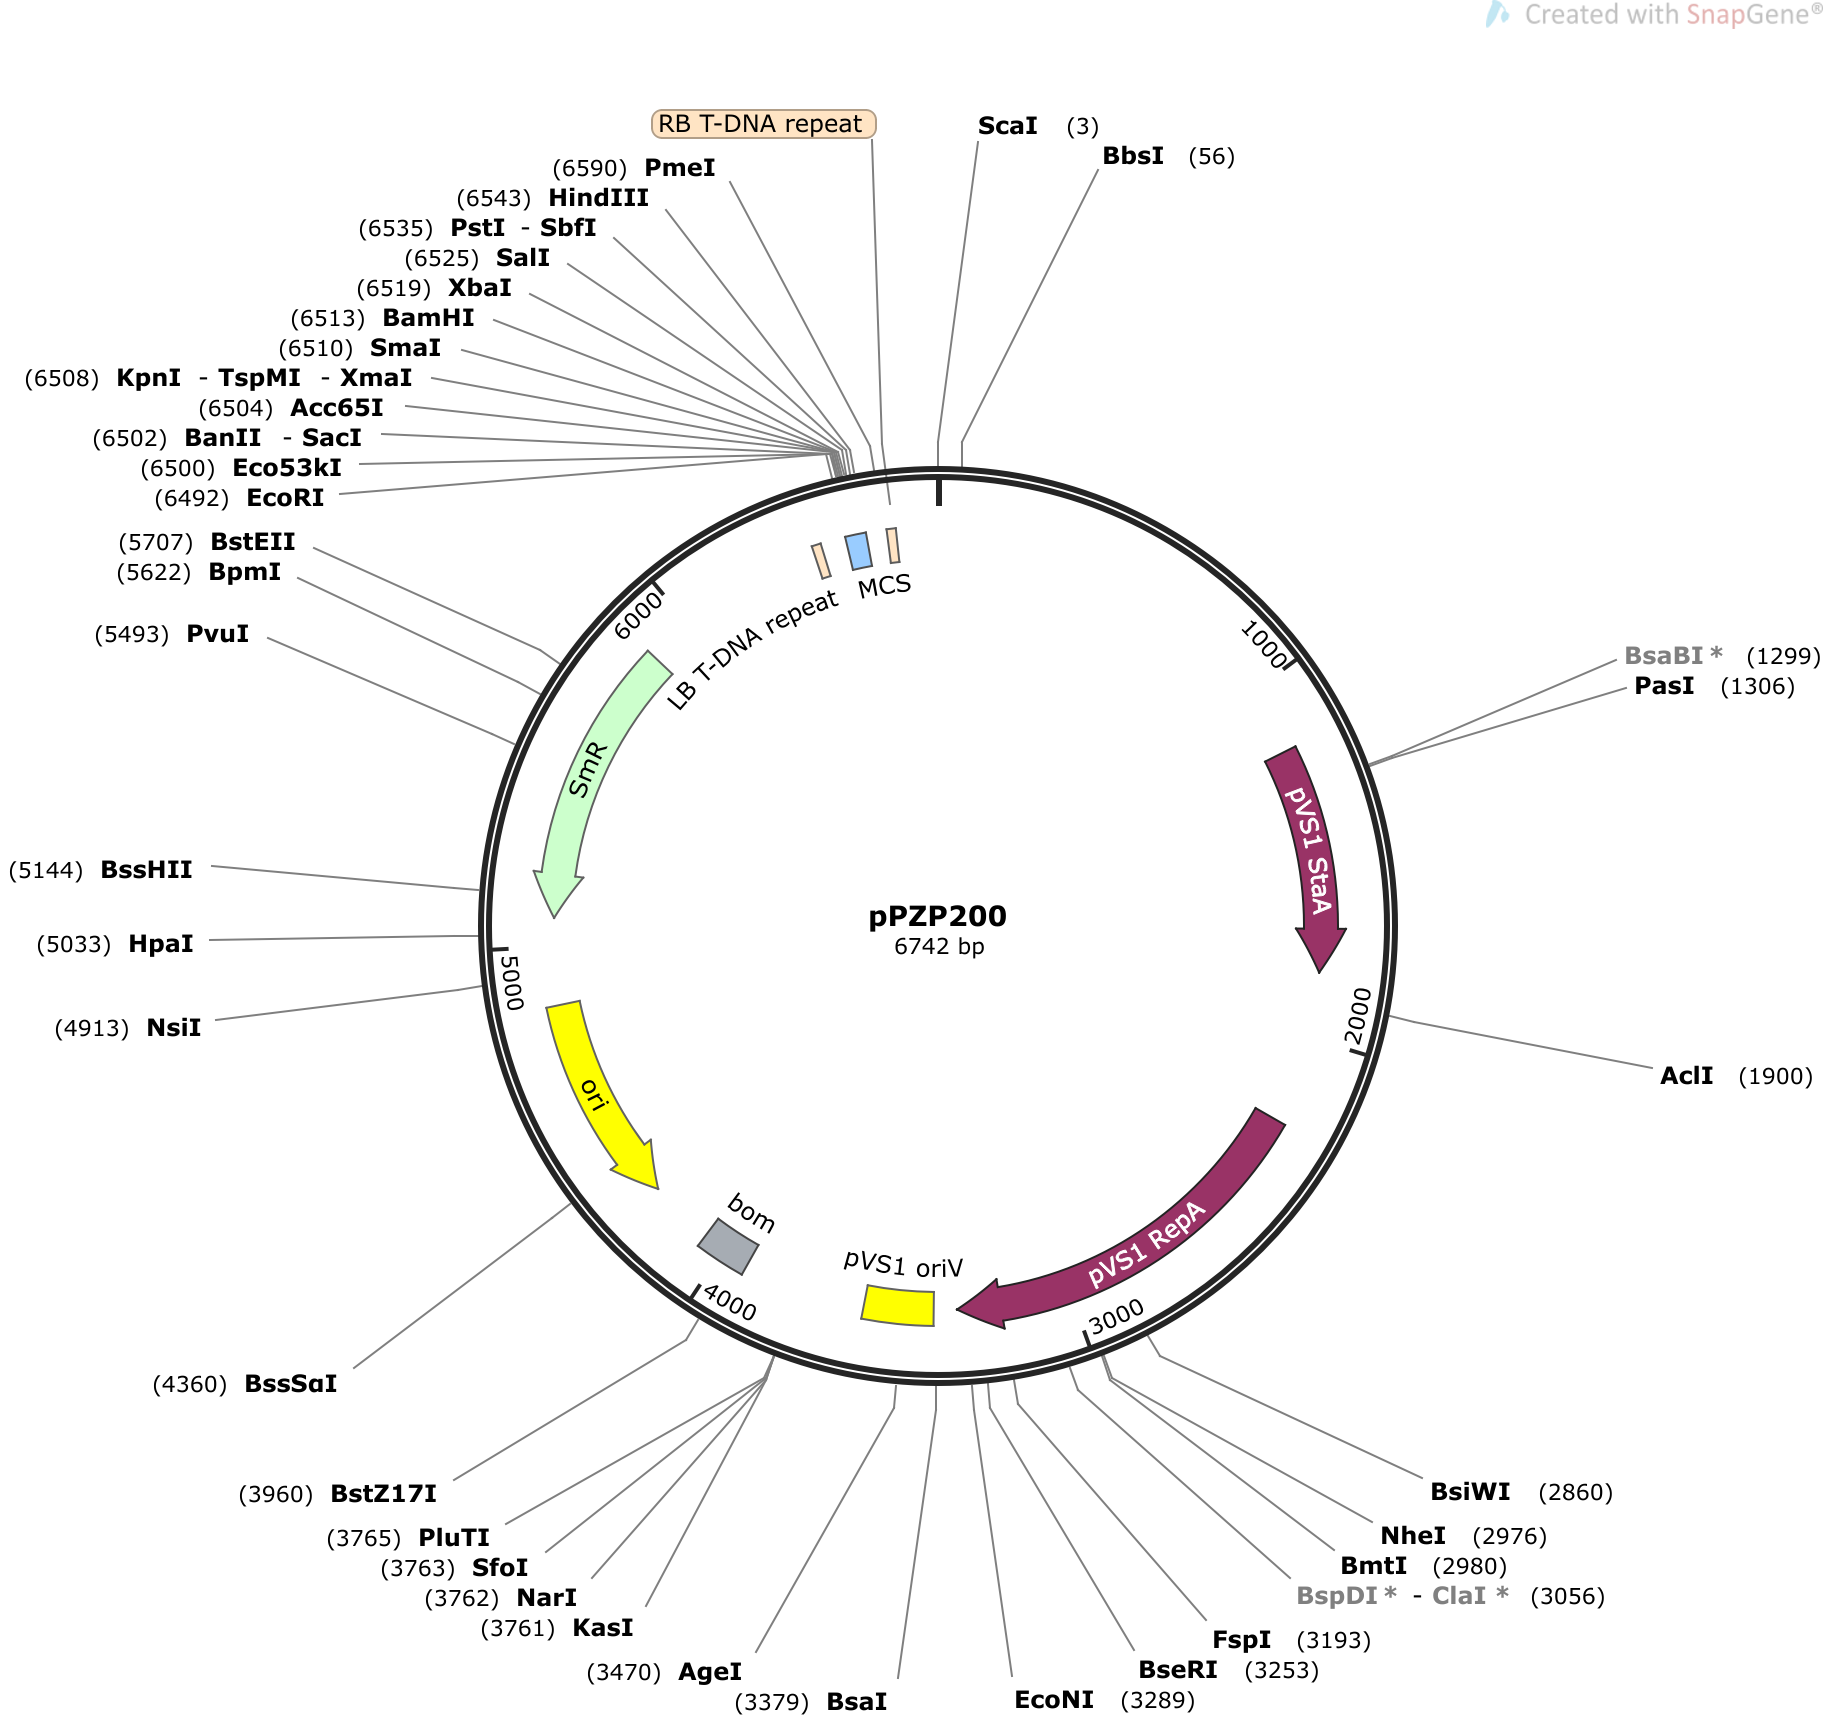
\includegraphics[width=\textwidth]{./figures/pPZP200.png}
		\caption{Wektor pPZP200}\label{fig::pPZP200}
		\end{subfigure}
		 \caption{Wektory użyte do stworzenia konstruktu AtU6-sgRNA-2 x 35S-Cas9}\label{fig::vectors}
	\end{tcolorbox}
\end{figure*}

\subsection{Otrzymanie konstruktu z genem RB}

Konstrukt pCLD04541 z genem RB i jego natywnym promotorem otrzymano od dr Jiming Jiang\autocite{Song2003}

\subsection{Transformacja pomidorów}

Obydwa uzyskane binarne wektory (gRNA-ekson2 i gRNA-ekson3) oraz konstrukt pCLD04541 z genem RB zostały wprowadzone do bakterii \textit{A. tumefaciens} szczep GV3101, za pomocą elektroporacji. Elektroporowane komórki były następnie inkubowane na medium LB suplementowanym spektynomycyną i streptomycyną, aby wyselekcjonować komórki, które przyjęły konstrukt.

Bakterie po namnożeniu zostały użyte do wprowadzenia kontruktów metodą leaf-disk\autocite{McCormick1986}, analogicznie do tego jak zostało to wykonane przez Pan'a \textit{i wspł.}\autocite{Pan2016}. Wysterylizowane nasiona były hodowane na 1/2 MS0. Po 6-8 dniach rosnące kotyledony zostały pocięte na nieduże kwadraty (<10mm), które zostały umieszczone na płytce z \textit{Agrobacterium}. Eksplantaty były następnie inkubowane z higromycyną dopóki z kallusów nie zregenerowały się dojrzałe rośliny. Ukorzenione rośliny zostały przesadzone do doniczek i przeniesione fotoperiodycznej komory wzrostowej.

\begin{figure}[tp]
\begin{tcolorbox}
	\centering
	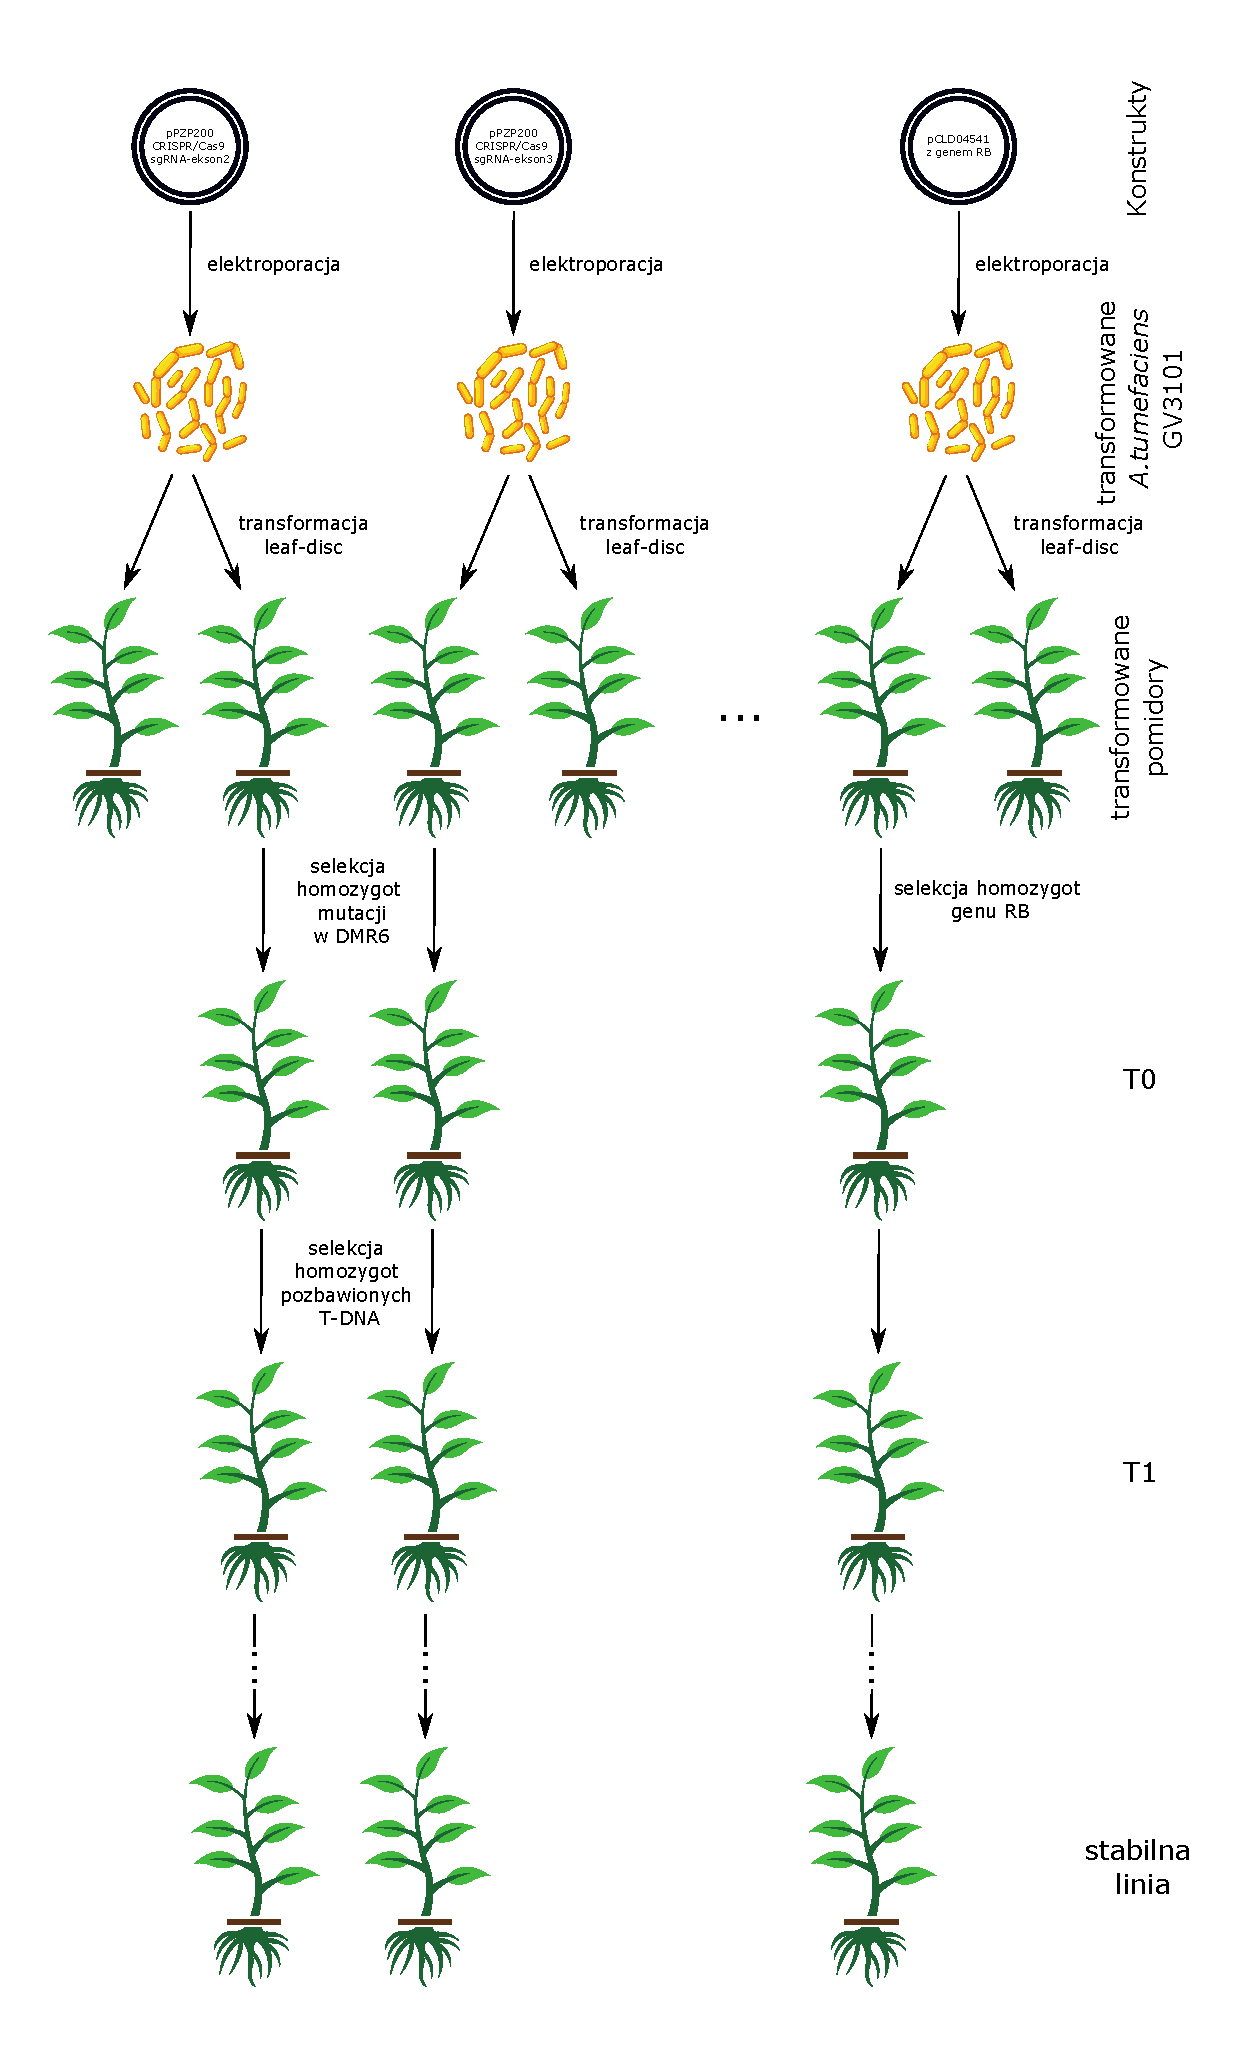
\includegraphics[width=0.96\textwidth]{./figures/scheme.pdf}
	\vspace{-2em}
	\caption{Otrzymane konstrukty zostały za pomocą elektroporacji wtransformowane do bakterii \textit{A .tumefaciens}. Bakterie zostały użyte do transformacji pomidorów. Z transformowanych roślin wybrano takie, które przyjęły T-DNA i oznaczono je jako pokolenie T0. Prowadzono selekcje aż do uzyskania stabilnych linii. (dla uproszczenia na rysunku pokazano mniej linii niż zostało otrzymanych)}
\end{tcolorbox}
\end{figure}

Uzyskane w ten sposób transgeniczne rośliny z CRISPR/Cas9 lub genem RB, oznaczono odpowiednio T0-CRISPR/Cas9 lub T0-RB, a ogólnie pokoleniem T0.

\subsection{Genotypowanie otrzymanych linii}

Z każdej rośliny z pokolenia T0 wyizolowane zostały próbki genomowego DNA z liści, łodyg i pąków. Dla T0-CRISPR za pomocą PCR zamplifikowano sekwencje targetowane przez odpowiednie gRNA oraz rejon T-DNA. Dla T0-RB zamplifikowano przy pomocy PCR tylko rejon T-DNA. Uzyskane na drodze amplifikacji fragmenty zostały wklonowane do wektorów pGEM (pGEM$^{\text{\textregistered}}$-T Easy Vector Systems, \textsf{Promega}) i następnie poddane sekwencjonowaniu. Fragmenty amplifikowane z sekwencji targetowanych przez CRISPR/Cas9 zostały dodatkowo poddane procedurze wykrycia mutacji przy pomocy zestawu EnGen$^{\text{\textregistered}}$ (EnGen$^{\text{\textregistered}}$ Mutation Detection Kit, \textsf{NEB}).

\subsection{Otrzyamanie stabilnych linii}

Rośliny homo- i heterozygotyczne pod kątem T-DNA (i mutacji w docelowym DNA dla T0-CRISPR/Cas9) zostały wyselekcjonowane z pokolenia T0 i skrzyżowane ze sobą w obrębie grup. Wybrane osobniki z pokolenia T1 poddano genotypowaniu w celu określenia dziedziczenia się mutacji i T-DNA.

\textbf{Dla linii CRISPR/Cas9 z wyciszeniem genu DMR6}. Z pokolenia T1 wyselekcjonowano homozygotyczne pod kątem mutacji w genie DMR6 i pozbawione T-DNA rośliny. Osobniki te zostały dalej ze sobą skrzyżowane.

Proces krzyżowania powtarzano aż do otrzymania stabilnych pod względem konkretnej mutacji w genie DMR6.

\textbf{Dla linii RB}. Wyselekcjonowano osobniki homozygotyczne pod względem transgenu. Osobniki te dalej ze sobą skrzyżowano w obrębie linii.

Proces krzyżowania powtarzano aż do utworzenia stabilnych pod względem transgenu linii RB.

\begin{figure}[tp]
\begin{tcolorbox}
	\centering
	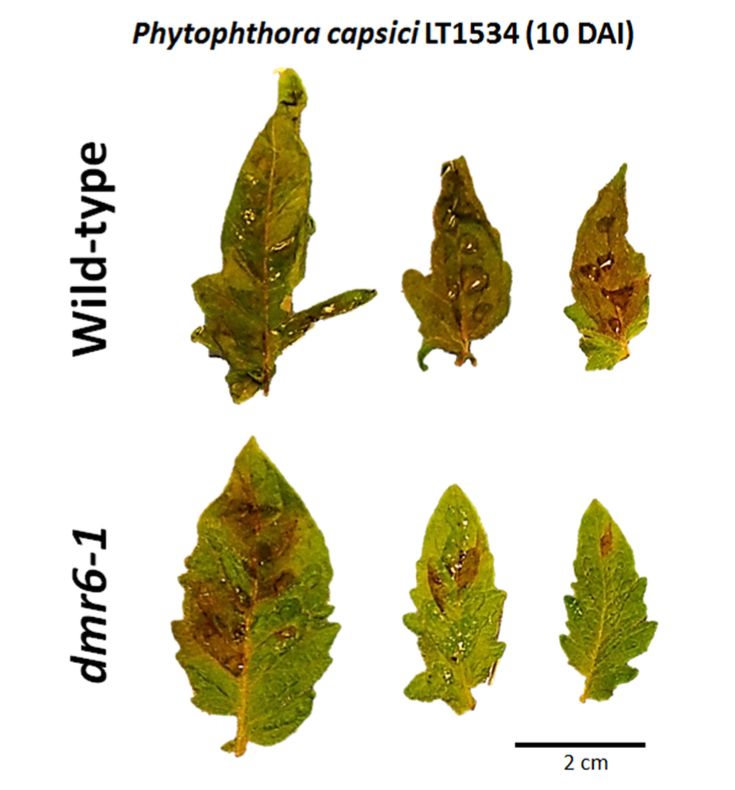
\includegraphics[width=\textwidth]{./figures/P_capsici_infection.png}
	\caption{Odmiana dzika (Wild-type) i mutant z wyciszonym genem DMR6 (dmr6), 10 dni po infekcji. Widoczne zmiany nekrotyczne -- silniejsze na odmianie dzikiej. (Na podstawie de Toledo Thomazella 2016)\autocite{deToledoThomazella2016}}\label{fig::p_capsici_infection}
\end{tcolorbox}
\end{figure}


\subsection{Określenie odporności poszczególnych linii na infekcję \textit{Phytophthora capsici}}

Rośliny ze stabilnych linii były hodowane w doniczkach ze zwykłą ziemią doniczkową w szklarniach, w temperaturze 25-30\degree C. Dwa razy dziennie odnotowywana była wysokość roślin.

Do oceny odporności na patogen użyty został szczep \textit{Phytophthora capsici} (ATCC$^{\text{\textregistered}}$ 15427\_TT™), hodowany według zaleceń zamieszczonych na stronie ATCC\autocite{ATCC} przez trzy dni w ciemności. Zawiesina spor została uzyskana poprzez płukanie wodą, porośniętych grzybnią płytek. Otrzymana w ten sposób zawiesina została rozcieńczona aż do otrzymania stężenia $10^{5}$ spor/ml.

Następnie liście wybranych roślin z poszczególnych linii zostały zakropione zawiesiną zoospor \textit{P. capsici}. Na każdy liść nakropiono taką samą objętość zawiesiny.

\subsection{Ocena stopnia odporności}

Jako kryteria do oceny stopnia odporności uzyskanych linii na patogen wybrano zmianę tempa wzrostu rośliny w stosunku do tempa przed infekcją, obecność i średnicę zmian na liściach (Fig. \ref{fig::p_capsici_infection}) oraz oraz stosunek średniej długości korzeni przybyszowych do długości korzenia głównego\autocite{Lamour2012}.

Wysokość rośliny była mierzona raz na 24h przez 10 dób. Rośliny były przez 10 dób obserwowane pod kątem obecności zmian na liściach i w razie średnica takich zmian była mierzona. Po 10 dobach obserwacji rośliny zostały wyciągnięte z ziemi i zmierzone zostały ich korzenie. Odnotowano także, czy charakterystyczne patologiczne zmiany wystąpiły na korzeniach.

\subsection{Linie kontrolne}

Oprócz opisanych wyżej transformowanych linii, z roślin transformowanych pozbawionym insertu plazmidem pPZP200 otrzymano linię negatywną, a z roślin nietransformowanych uzyskano linie podwójnie negatywną. Wyniki mierzenia stopnia odporności dla pozostałych linii były odnoszone do wyników jakie odnotowano dla roślin z linii negatywnej i podwójnie negatywnej po zakażeniu patogenem.

\section{Dyskusja}

Otrzymanie roślin odpornych na patogeny z rodzaju \textit{Phytophthora} stanowi duże wyzwanie ze względu na wysoką zmienność organizmów w tym taksonie. Trwają próby wytworzenia odmian odpornych na patogeny z tego rodzaju. Badania te mają ogromne znaczenie gospodarcze ze względu na wysokie straty powodowane w uprawach przez wywoływane przez \textit{Phytophthora} choroby\autocite{Lamour2012, Barchenger2018, Sy2005, Chen2019, Song2003, Bagga2019}.

Z powodu braku literatury związanej z otrzymywaniem linii pomidorów odpornych na \textit{Phytophtora capsici} w niniejszym projekcie opisano metodę otrzymania stabilnej linii pomidora i zbadanie jej odporności na patogen, ale nie podano konkretnych wyników. W zamian za to zamieszczono odniesienia do analogicznych badań. Opisane tutaj metody służą otrzymaniu odmiany pomidora, która potencjalnie może wykazywać odporność na infekcje \textit{P. capsici}, i ocenie, który z dwóch zaproponowanych sposobów (CRISPR/Cas9 KO genu DMR6 i transformacja genem RB z \textit{Solanum bulbocastanum}) daje w efekcie rośliny o trwalszej i większej odporności.

Prócz genów DMR6 i RB na odporność/podatność ma także potencjalnie gen SlROS-II.1, którego Knockout powoduje zwiększenie podatności na infekcje \textit{P. capsici}\autocite{Yang2020}. Kolejną potencjalną metodą uzyskania odpornych roślin jest więc wywołanie trwałej lub warunkowej nadekspresji tego genu.

Opisano tutaj użycie dwóch potencjalnych metod uzyskania odpornych na \textit{P. capsici} odmian pomidora i podkreślono etap otrzymania stabilnych pod kątem interesującego nas genu linii, co nie zostało poruszone w cytowanych na początku pracach, które skupiały się w znacznej mierze na samym zagadnieniu odporności.

\printbibliography

\end{document}
